\section{FluidGeneratorAgent LLM Based}

\subsection{Introduction and Defitions}

Large Language Models (LLMs) can do several tasks, due to the large amount of data on they are trained. In the paper \textit{Language Models are Few-Shot Learners} (Brawn et al. 2020), the authors presented three different ways to improve the results of LLMs in specific tasks, without doing any \textit{fine-tuning}. We refer to these techniques as \textit{prompting strategies}. Before describing the three different prompting strategies, it is important to give some definitions.

\textbf{Definition 1: Example}. In the context of LLM, an \textit{Example} $E$ is a pair $(Q, A)$ where $Q$ is an object which contains the input for the LLM; $A$ is an object with contains the answer generated by the LLM.

\begin{figure}[!h]
    \centering
    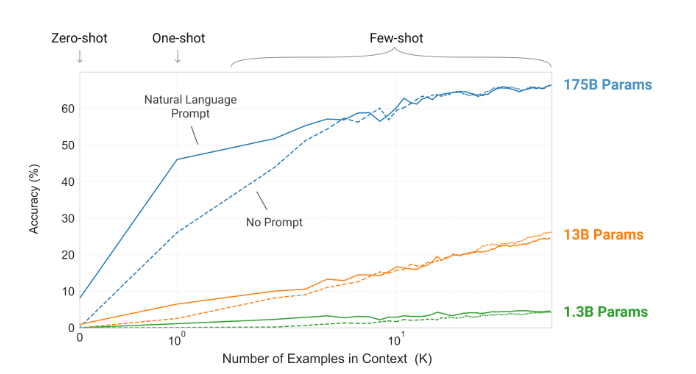
\includegraphics[width=1\linewidth]{fig/image.png}
    \caption{Larger models make increasingly efficient use of in-context information [from Brown paper]}
    \label{fig:enter-label}
\end{figure}

\textbf{Definition 2: Prompt}. In the context of LLM, a \textit{Prompt} $P$ is a pair $(C, E*)$ where $C$ represents the \textit{context} description for the task that the LLM has to perform, while $E*$ represents a list of Examples (zero or more examples).

The \textit{context} in the prompt is important, because it describes the task in which the LLM is involved, through a description that is in Natural Language (NL).

Figure \ref{fig:enter-label} highliths that the significance of $C$, in given $P$ prompt, decrease when $|E*|$ increases. Given \( E^* \) (a set), a list of prompts, and \( C \) (a context) and \textit{Relevance} a function which measure the impact of a text in the accuracy:

\[
|E^*| \to \infty \implies \text{Relevance}(C) \to 0.
\]

\subsection{Informal Design}

In this section, a description of the workflow we will implement is given. The goal of the system is mainly to generate parts of a Fluid program. In particular, starting from a textual input, like a caption, we want to replace in the caption the parts that could be generated by Fluid functions.

\begin{table*}[!ht]
    \centering
    \caption{Examples}
    \begin{tabular}{p{13cm}}
    \hline
    \hline
    \\\textbf{Input}:\\
    The SSP1-2.6 scenario caps an increase to $v1$ by the century's end, with an exceedance being unlikely. Contrastingly, SSP2-4.5 considers it likely.\\\\
    \hline
    \\\textbf{Output}:\\
    "The ", sspone.scenario, " scenario caps an increase to ", numToStr sspone.bestE81100, " by the century's end, with an exceedance being ", likelihoodMap(findLikelihood(sspone.low81100, sspone.high81100) 2.0), ". Contrastingly, ", ssptwo.scenario, " considers it ", likelihoodMap(findLikelihood(ssptwo.low81100, ssptwo.high81100) 2.0), "."\\
    \hline
    \hline
    \end{tabular}
\end{table*}

To achieve the results described above, we designed the following system architecture. Figure \ref{fig:fluid-llm-architecture} illustrates the proposed architecture.
The process begins with the input object being passed to the Recognition Agent, which analyzes the input, identifies elements to be replaced, and substitutes them with tags. The tagged content is then forwarded to the FluidGenerator Agent, which replaces the tags with the corresponding functions.
The output from this process is sent, along with the input, to the Validation phase. During this phase, the Replacing Validator ensures that changes were made exclusively to the tags. Additionally, the Parser Agent executes the generated code to validate the results.
If either validation step fails, the errors are returned to the FluidGenerator Agent for iterative correction and refinement.

\begin{figure}
    \centering
    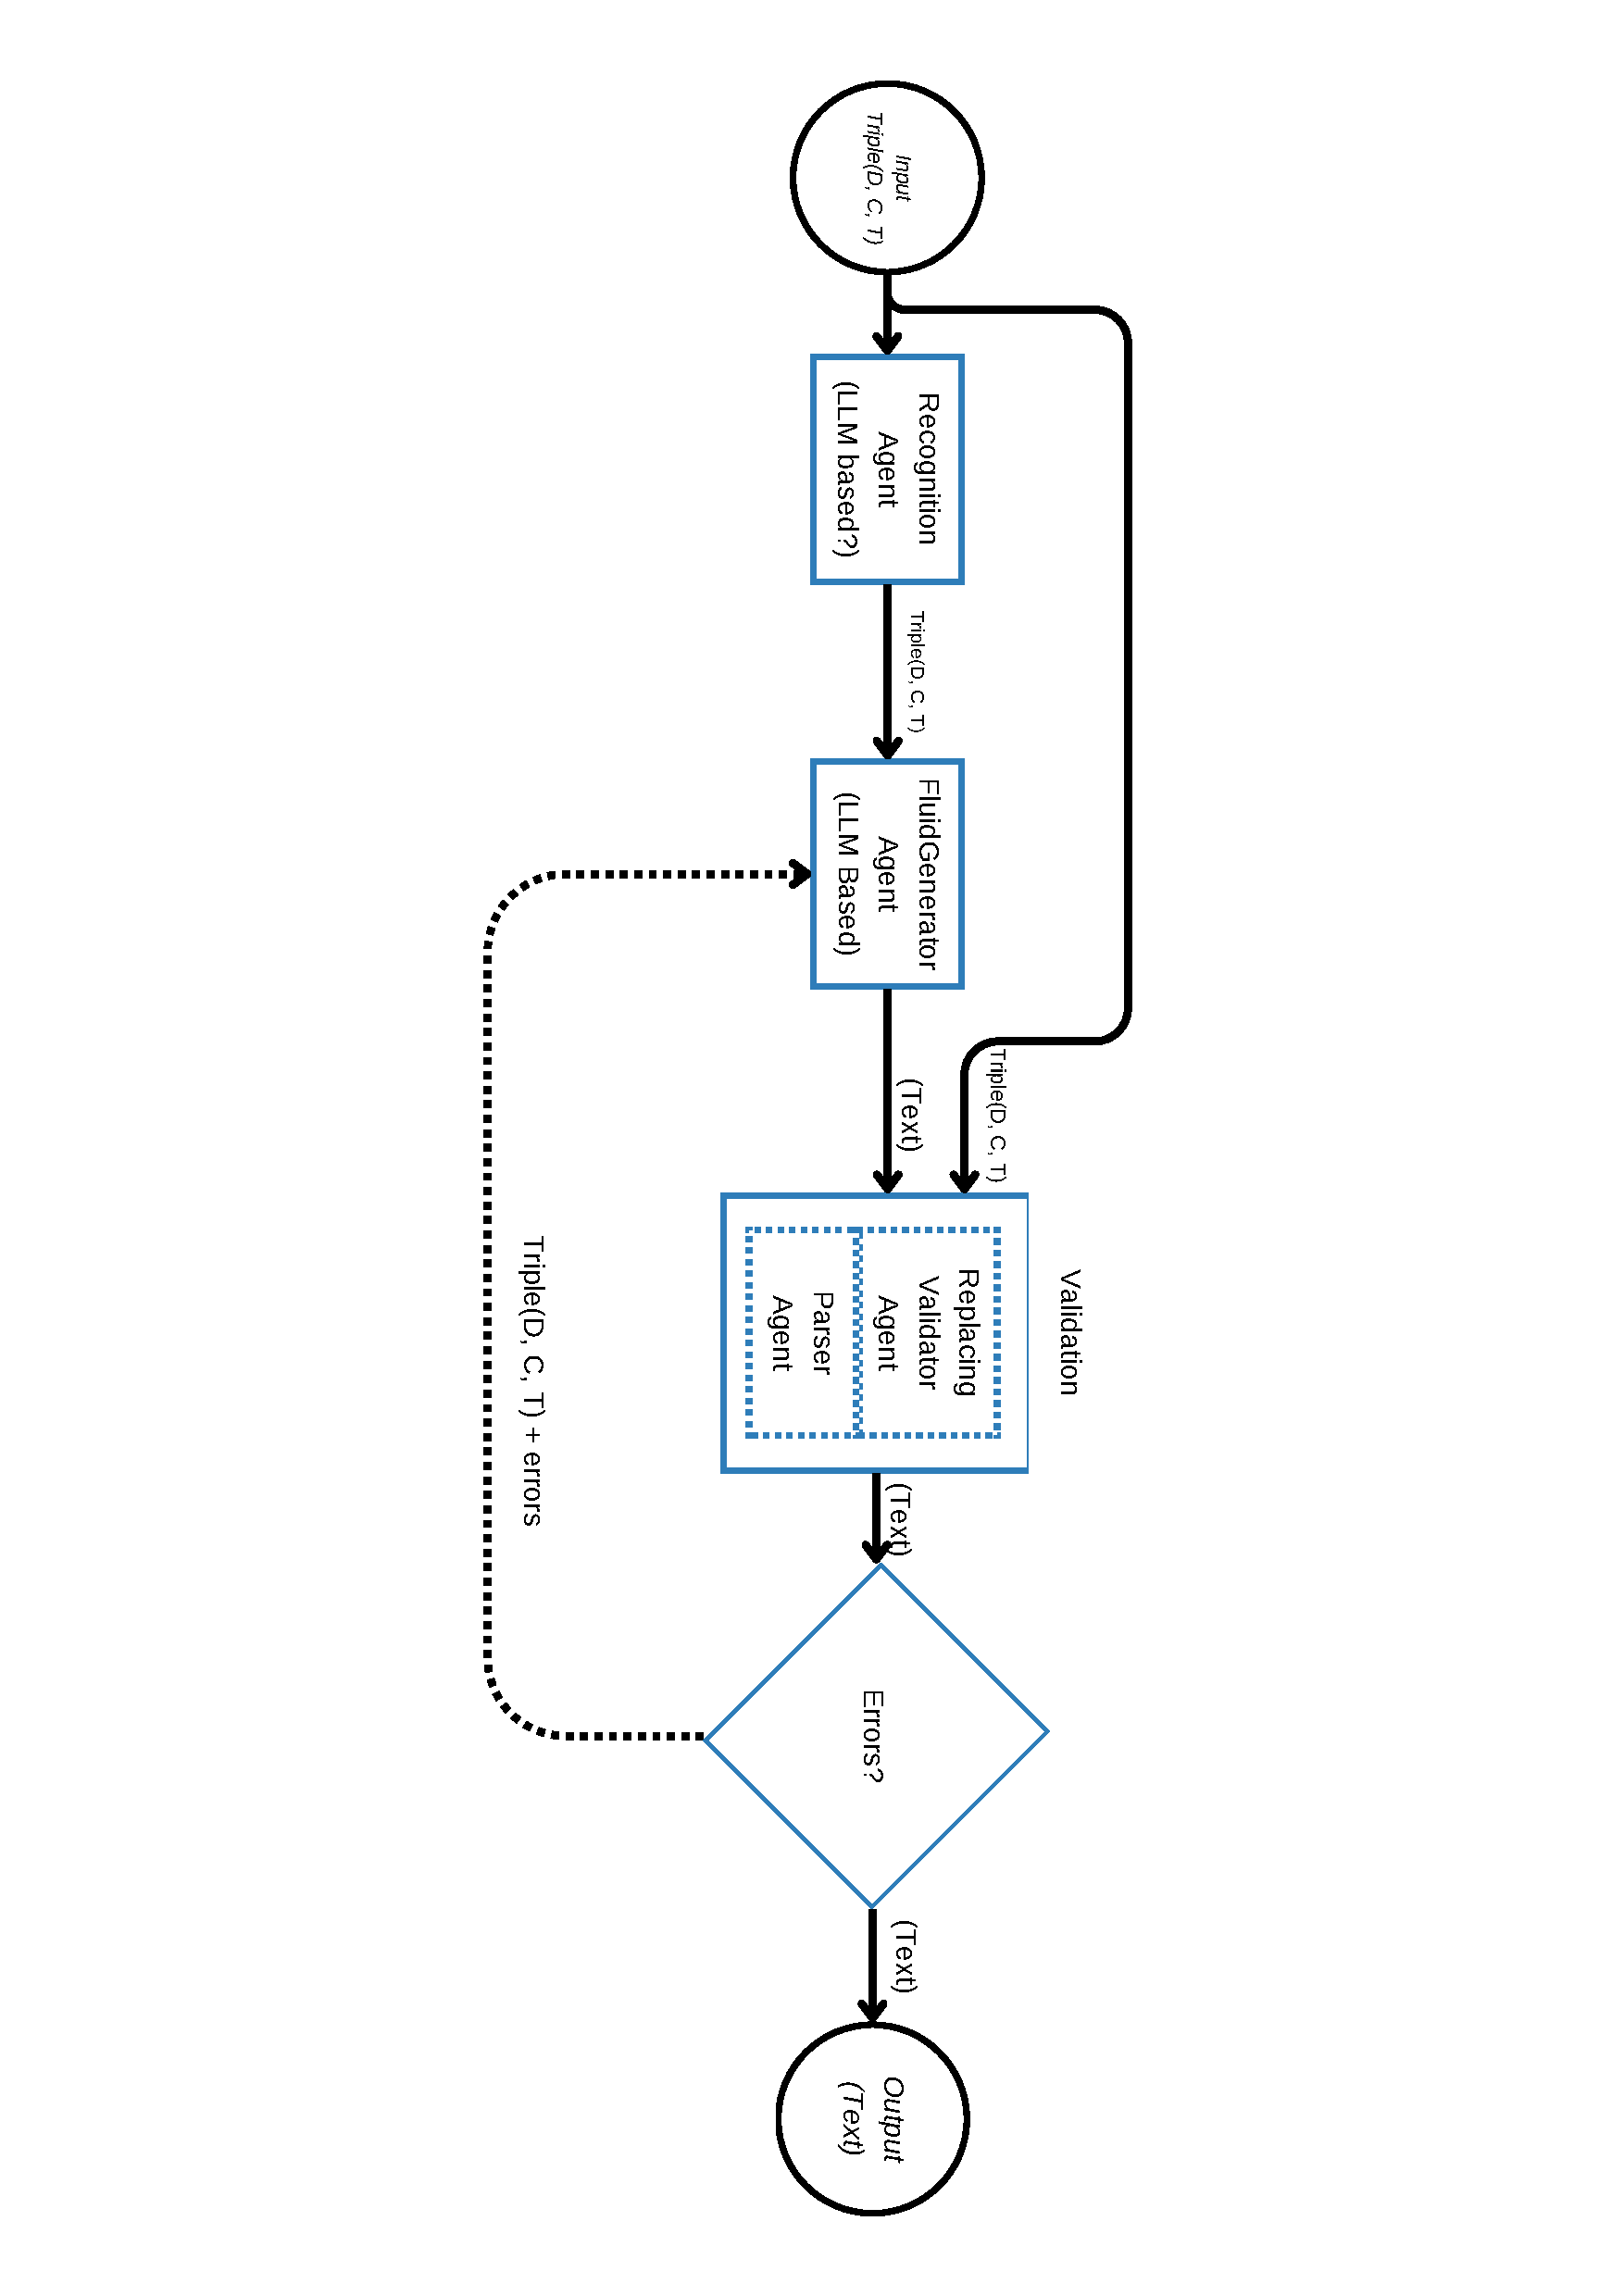
\includegraphics[width=1.2\linewidth]{fig/fluid-llm-architecture.pdf}
    \caption{Draft architecture of the system}
    \label{fig:fluid-llm-architecture}
\end{figure}

\subsubsection{Input}
The input for this system needs to describe the following information:
\begin{itemize}
    \item \textbf{Data}: the data that the fluid program is using in the program. This data have a JSON-like format.
    \item \textbf{Fluid Code}: Parts (or entire) Fluid program, used to link the variables to the text
    \item \textbf{Text}: text element that the system will work on, replacing informations that can be extracted from variables or functions with the relate fluid elements.
\end{itemize}

Given the necessity to provide to the system both the content and its meaning, these informations will be passed to the system through a JSON string which has to respect the schema reported in Table \ref{tab:schema_fluid_input}.

\begin{table*}[!ht]
    \centering
    \caption{Input JSON Schema \label{tab:schema_fluid_input}}
    \begin{tabular}{p{13cm}}
    \hline
    \hline
    \begin{verbatim}
{
  "$schema": "http://json-schema.org/draft-04/schema#",
  "type": "object",
  "properties": {
    "data": {
      "type": "string"
    },
    "code": {
      "type": "string"
    },
    "caption": {
      "type": "string"
    }
  },
  "required": [
    "data",
    "code",
    "caption"
  ]
}
    \end{verbatim}\\
    \hline \hline
    \end{tabular}
\end{table*}

\begin{table*}[!ht]
    \centering
    \caption{Input JSON Example \label{tab:json_fluid_input}}
    \begin{tabular}{p{13cm}}
    \hline
    \hline
    \begin{verbatim}
{
    "data": "[
    { scenario: "SSP3-7.0", bestEst2140: 1.5, low2140: 1.2, high2140: 1.7, bestEst4160:
    1.6, low4160: 1.2, high4160: 2.0, bestEst81100: 1.4, low81100: 1.0, high81100: 1.8},
    { scenario: "SSP1-1.9", bestEst2140: 1.4, low2140: 1.2, high2140: 1.8, bestEst4160:
    2.0, low4160: 1.6, high4160: 2.5, bestEst81100: 2.7, low81100: 2.1, high81100: 3.5}
    ]",
    "code": "let envDataTable = newDataTable 13;\n    probMetric = newModel 0.35;\n
    earlyScenario = getByScenario \"SSP3-7.0\" envDataTable;\n    lateScenario =
    getByScenario \"SSP1-1.9\" envDataTable",
    "caption": "The scenario SSP3-7.0 outlines a more substantial risk, rendering the
    chance of exceeding the 2°C mark more likely than not. Meanwhile, SSP1-1.9 charts a
    different course, with a restrained 1.4 rise, making such an exceedance very unlikely."
  }
\end{verbatim}\\
    \hline \hline
    \end{tabular}
\end{table*}

\subsubsection{Recognition Agent}
The Recognition Agent role is \textit{identify} the parts in the input that need to be processed to the \textit{FluidGenerator Agent}. In particular, there are three categories that need to be replaced:
\begin{itemize}
    \item \textbf{Scenario names}. Name of the scenario that the text is descring.
    \item \textbf{Data values}. Values in the text that are reported in the \textit{data} part of the input.
    \item \textbf{Function outputs}. Values that could be computed by a function (like \textit{likelihoodMap} function, for statistical phrases like \textit{likely}.
\end{itemize}

The Recognition Agent replaces the text with a tag in order to give the FluidGenerator Agent the indications about where it has to work.

\paragraph{Implementation Details}
This agent can be implemented through a Large Language Model (like llama3, gpt-3.5 or gpt\-4o) or also through a specific model that will be trained.

\subsubsection{FluidGenerator Agent}.
The \textit{FluidGenerator Agent} has to replace the tag from the input with the respective variables or function calls. For example, if the input contains the tag \textbf{[SCENARIO\_NAME value='SSP1-2.6']}, the agent replaces the tag with the variable that generates the string in the value attribute. Table \ref{tab:agent_execution_sample} describes the input, the results of the Recognition Agent (in the \textit{Input after Recognition Agent} part), and the expected output after the FluidGenerator Agent execution.

\begin{table*}[!ht]
    \centering
    \caption{How the input changes through the Agent Executions \label{tab:agent_execution_sample}}
    \begin{tabular}{p{13cm}}
    \hline
    \hline
    \\\textbf{Input}:\\
    \begin{verbatim}
        {
            "data": [{"scenario": "SSP1-2.6", "low": 1, "high": 2}],
            "code": "let realTable = newDataTable 3;
                         probTable = newModel 0.3;
                        sspone = getByScenario "SSP1-2.6" realTable;",
            "caption": "For SSP1-1.9, the rise in global temperature
                        by century's end is contained at 2."
        }
    \end{verbatim}
    \\
    \hline
    \\
    \textbf{Input after Recognition Agent}
    \begin{verbatim}
        {
            "data": [{"scenario": "SSP1-2.6", "low": 1, "high": 2}],
            "code": "let realTable = newDataTable 3;
                         probTable = newModel 0.3;
                        sspone = getByScenario "SSP1-2.6" realTable;",
            "caption": "For [SCENARIO_REPLACE value='SSP1-1.90, the rise in
                        global temperature by century's end
                        is contained at [NUM_REPLACE value='2']."
        }
    \end{verbatim}\\
    \hline
    \\\textbf{Expected Output after FluidGenerator Agent}:\\
    \begin{verbatim}
        "For ", sspone.scenario, ", the rise in global temperature
        by century's end is contained at ", numToStr sspone.high, "
    \end{verbatim}

    \\
    \hline
    \hline
    \end{tabular}
\end{table*}

\subsubsection{Validation Phase}
In the Validation Phase, the system checks the output of the FluidGenerator Agent, through two strategies.
\begin{enumerate}
    \item The "Replacing Validator Agent" verifies that the previous agent only modified the values identified by the tags.
    \item The "Parser Agent" executes the generated output in order to check that the results is equal to the input text.
\end{enumerate}

If one of these checks fails, the generated output and errors are passed back to the Fluid Generator agent, which will also take into account the error messages generated by these two agents.

\subsubsection{Output}

At the end of this pipeline, we have the generated output, which is a string like the one reported in Table \ref{tab:agent_execution_sample}.
